\documentclass[12pt]{article}
\usepackage[utf8]{inputenc}
\usepackage{subcaption}
\usepackage{graphicx}
\usepackage{float}
%\usepackage[
%top    = 0.25cm,
%bottom = 0.25cm,
%left   = 1.00cm,
%right  = 1.00cm]{geometry}
\usepackage[margin=1in]{geometry}

\title{ECS171 Final Report}
\author{Team 4}
\date{December 5, 2021}

\begin{document}

\maketitle

\newcommand{\CVItemListStart}{\begin{itemize}}
\newcommand{\CVItemListEnd}{\end{itemize}\vspace{-5pt}}
\newcommand{\TimelineStart}{\begin{itemize}}
\newcommand{\TimelineEnd}{\end{itemize}\vspace{-5pt}}

\section{Team Members}
Leader: Kyle Ross\\
Group Members: Stephen Wong, Thalia Fay, Shawn Headley, Haley Chung, Yu Lai, Adarsh Pantula, Jie Shao, Bryce Naung, Fangjing Li, Yuhao Zhuang.\\

\noindent Project Repository Link: https://github.com/StephenW789/ECS-171-FinalProject
\section{Introduction}
Our team chose the project to be on customers segmentation and analysis. The dataset of our choice, the 2021 Customer Personality Analysis Dataset available on Kaggle, had a wide range of customer data and the consumption of products.\\

\noindent When large corporations market products aggressively towards specific customer groups, they seek to perform customer segmentation. Customer segmentation is a process in which customers are divided up into segments such that the customers in each segment are similar to one another in some category (i.e. spending habits, interests, gender, age, etc.). \\

\noindent In the context of sales marketing, customer segmentation allows businesses to make better data-driven inferences about their customers’ needs/behaviors. Identifying why current customers chose a particular company's product over rival brands is critical. Once certain attributes are identified, they should be kept in mind for future releases, so current customers would remain loyal. Depending on a customer segment's characteristics, a business can modify their product to better suit the needs of their target customers.\\

\noindent Our group performed various unsupervised clustering techniques to compare and determine which technique would give us the best structure for the given dataset and allow us to segment the customer data into groups that are easily identified and profiled.\\

\noindent The goal of our project was to group similar customers and determine which attributes played a significant role in the customer segmentation. For instance, a question we had was what kind of customers purchased the highest amount of products in each product category.\\

\section{Literature Review}
Hung's and others' research focused on the usage of Agglomerative Clustering for customer segmentation using Credit Card datasets. Agglomerative Clustering was chosen over K-means because Agglomerative tends to provide better clusters. Agglomerative is more computationally expensive compared to K-means, but this difference will be negligable for smaller datasets  (Hung et al. 2019).\\

\noindent Within Shihab's and others' research, comparative analysis between K-means, Agglomerative Clustering, and Advanced K-means was performed. Advanced K-means used additional data structures to avoid unnecessary distance computation between object and centroid. This new technique outperformed regular K-means and Agglomerative Clustering by far. However, there were also notable differences between the latter two methods (Shihab et al. 2019).\\

\noindent The reason why Agglomerative outperforms K-means was due to fact that the former does not force the data into exactly k clusters in the early stages of the clustering. Rather, each data point starts off as its own individual "cluster". As the algorithm progresses, similar data points are slowly placed into one small cluster. Towards the end of the algorithm, the  many small clusters are agglomerated into exactly k-clusters (Shihab et al. 2019).\\


\noindent Ekhlassi's and others' research analyzed the relationship between customer personality and brand personality. A common marketing used by Big Tech, corporations build a certain "brand" of their product and market exclusively to customers whose personality, morals, and values align with that brand (Ekhlassi et al. 2012).\\

\noindent The research concluded a strong correlation between a conscientious customer valuing ethical corporations and the "social responsibility" of the brand image (Ekhlassi et al. 2012). \\

\noindent Our team's research will extend their research idea through analysis of individual attributes that affect customer purchases.\\

\section{Dataset Description}

Link: https://www.kaggle.com/imakash3011/customer-personality-analysis\\

\noindent The dataset contains 2240 rows of unlabeled data entries. The different columns in the dataset are split into 4 primary sections. The People section identifies each customer by education level, marital status, etc. The Products section lists the amount each customer has spent on different products such as meats, fruits, wines, etc. The Promotion section includes number of purchases made with discounts and which promotion deals were accepted by each customer. The Place section contains the number of purchases a customer has made from a specific medium, such as online versus in-store purchases.\\

\noindent At first glance, our group took note of some attributes listed under the People section that we believed would likely affect customer purchases. These included the customer's birth year, marital status, income, and education. However, we knew we needed to perform exploratory data analysis to determine which attributes were the most significant for customer segmentation. In addition, we decided to do some feature engineering after looking at the given attributes, such as calculating a customer's age based on their birth year.\\

\noindent We also noted that for the Promotions section, no information was given on what exactly the different deals offered to the customers were so we kept this in mind when performing our clustering (we removed some attributes from this section later on).\\

\noindent Lastly, we noticed that there were a few null values in the income column, which we made sure to remove in our data cleaning and pre-processing.\\

\section{Proposed Solution and Experimental Results}

Because we have an unlabeled dataset, our team applied four different unsupervised learning techniques to perform custom segmentation: Agglomerative Clustering, Apriori Algorithm, K-Means, and Fuzzy C-Means.\\

\noindent Before performing all of our unsupervised learning methods, the first thing we made sure to do was data cleaning and pre-processing. We dropped all rows that contained null values in the Income column, reducing the number of data entries from 2240 to 2216 entries. Next, we performed feature engineering by modifying certain existing attributes and creating new features using the given attributes. We simplified attributes that had repetitive values and removed redundant attributes/columns. We created new features for the age of the customer, total spending across all the different products, total number of children, and family size. During our data cleaning process, we created pairplots with notable attributes such as Income and Age to identify potential outliers. A few outliers were visually identifiable, such as income that was 600,000k or above and age that was over 90 years, so we removed them from the our cleaned dataset. Additionally, we encoded all of our categorical attributes using the label encoder and standardized our data.\\

\noindent Along with the new features we created, there were over twenty different attributes in our cleaned dataset. We created a heatmap for our dataset to visualize which attributes have high correlations with each other. We noticed that certain attributes did have relatively high correlation with each other, such as income and the amount spent on wine purchases. When two attributes have high correlation, this means that one of them is redundant so we decided to perform dimensionality reduction using principal component analysis (PCA) to help us with feature selection. Using a Scree Plot and some trial and error, we found that the optimal number of principal components to include was three.\\ 

\noindent To determine the optimal number of clusters for our clustering methods, we used the Elbow Technique for K-Means clustering. Along with some trial and error, we found that having four clusters gave us the most evenly distributed clusters and least overlap between clusters; thus, we had four clusters for all three of our clustering methods.\\

\noindent After running the different models, we created bar charts for multiple attributes to help us find similarities between the customers in each cluster. Some of the bar charts used for the profiling of the four clusters from K-Means clustering are shown in figures 1 and 2. We also plotted the consumption of the different product categories for each cluster in figure 4. From our results, the profiling of each cluster is as follows:
\begin{center}
    \begin{itemize}
      \item Cluster 0 are large families with middle aged parents often having multiple kids and teenagers. Having a large family leads to higher expenses.
      \item Cluster 1 are mostly high earning single individuals or childless couples.
      \item Cluster 2 are smaller families with lower earning young parents with mostly kids and very few teenagers.
      \item Cluster 3 are smaller families with high earning middle-aged parents and teenagers.
    \end{itemize}
\end{center}

\begin{figure}[H]
    \centering
    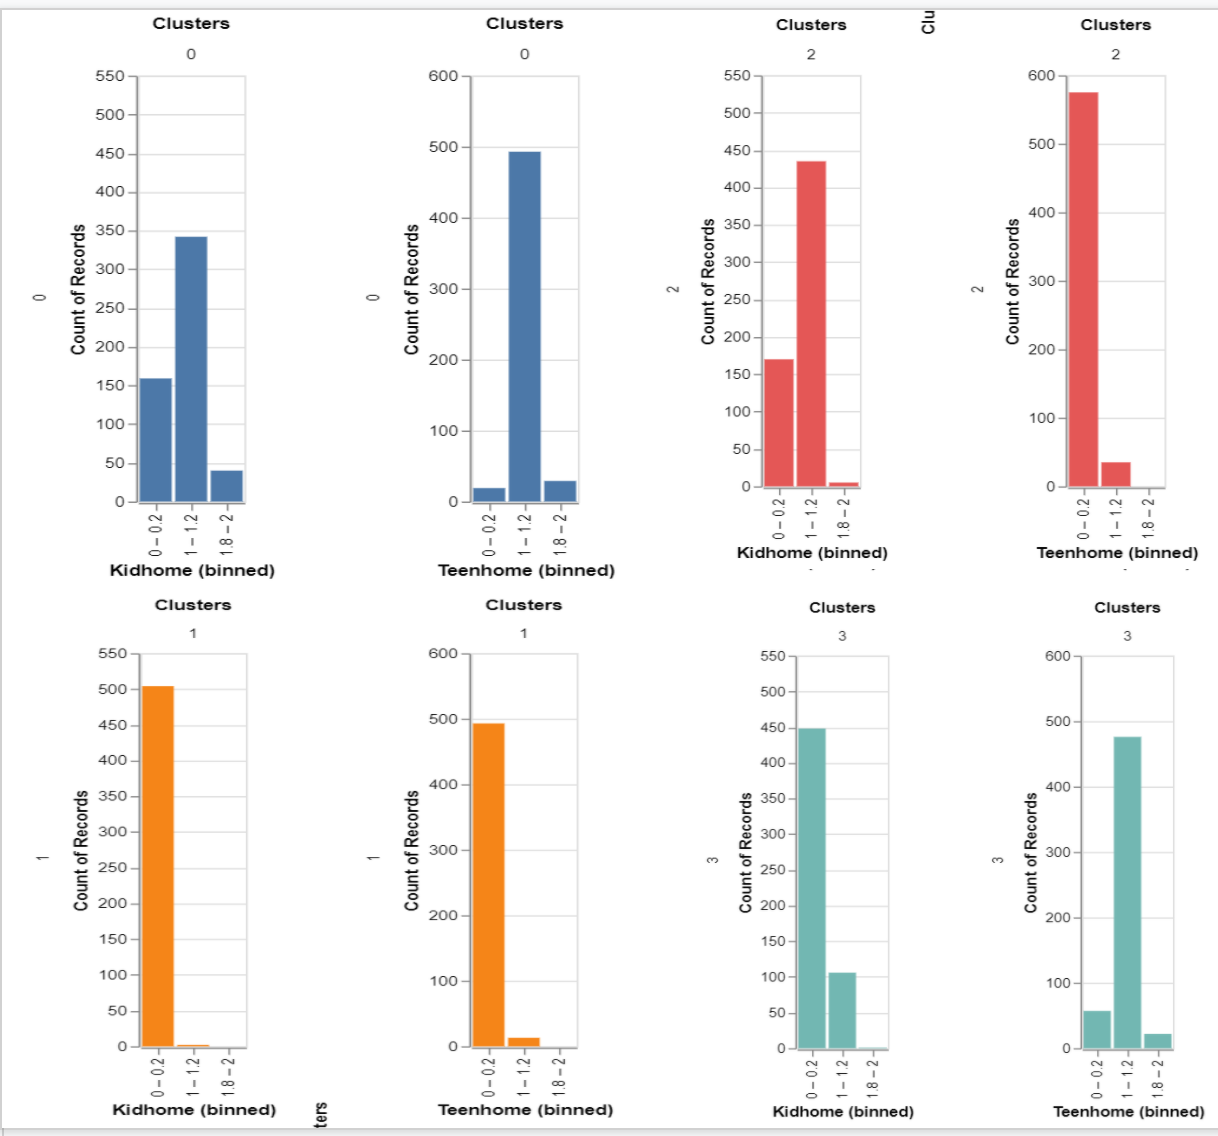
\includegraphics[scale = 0.25]{figures/Clusters_kids.png}
    \caption{Clusters 0 - 3 statistics}
\end{figure}
\begin{figure}[H]
    \begin{subfigure}{\textwidth}
        \centering
        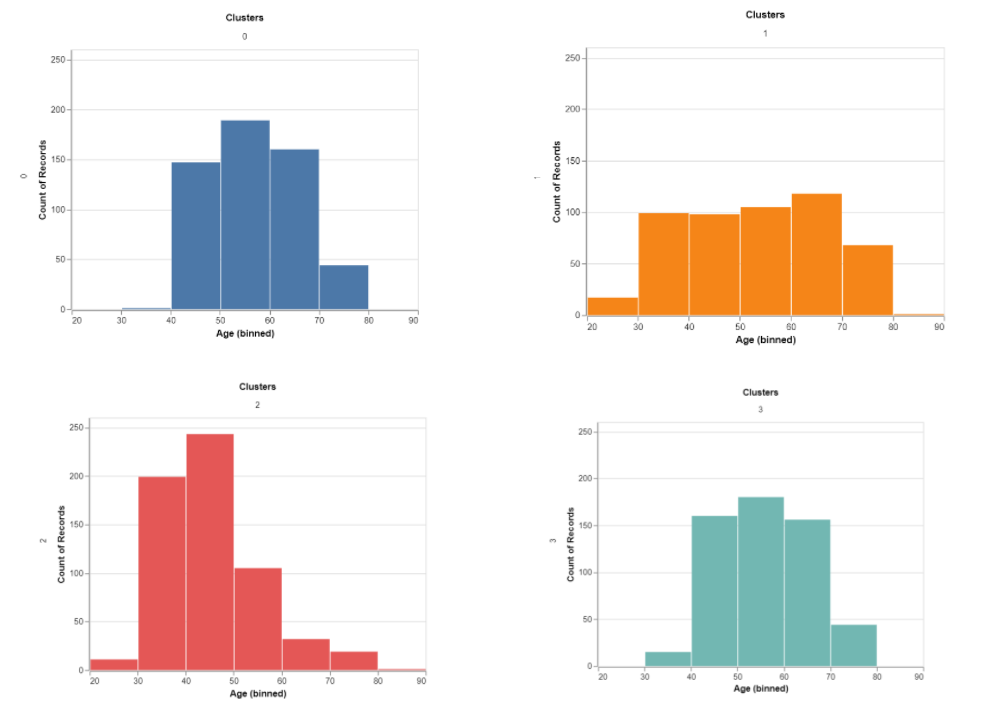
\includegraphics[height=7cm]{figures/Clusters_age.PNG}\hfill
    \end{subfigure}
    \newline
    \begin{subfigure}{\textwidth}
        \centering
        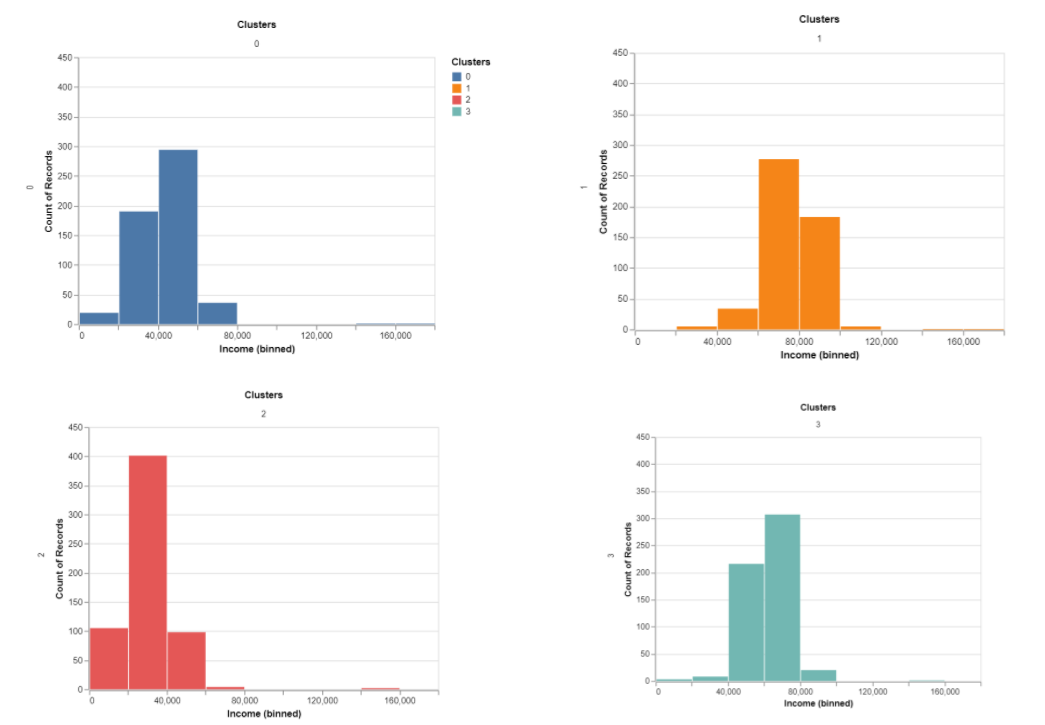
\includegraphics[height=7cm]{figures/Clusters_income.PNG}\hfill
    \end{subfigure}
  \caption{Clusters 0 - 3 statistics}
\end{figure}
\begin{figure}[H]
  \begin{subfigure}{\linewidth}
  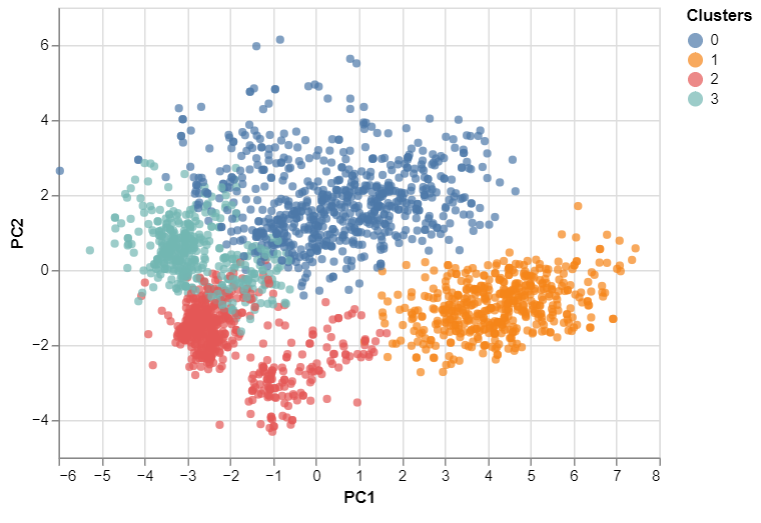
\includegraphics[width=.3\linewidth]{figures/Agglomerative_clusters.PNG}\hfill
  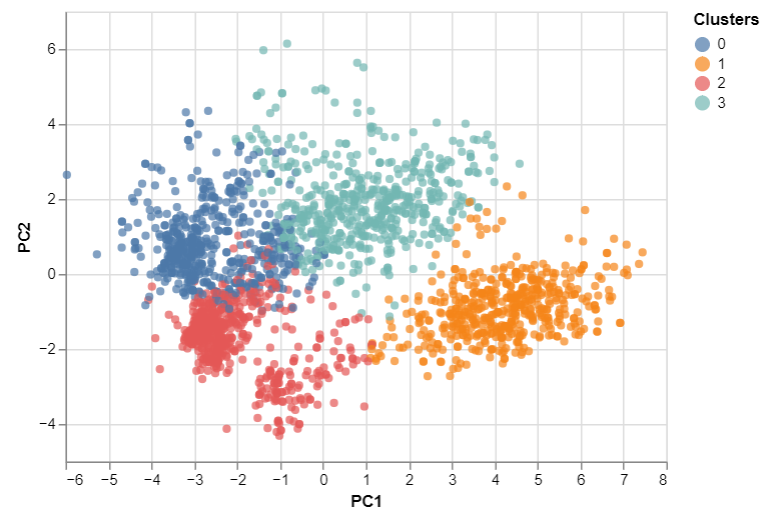
\includegraphics[width=.3\linewidth]{figures/KMeans_clusters.PNG}\hfill
  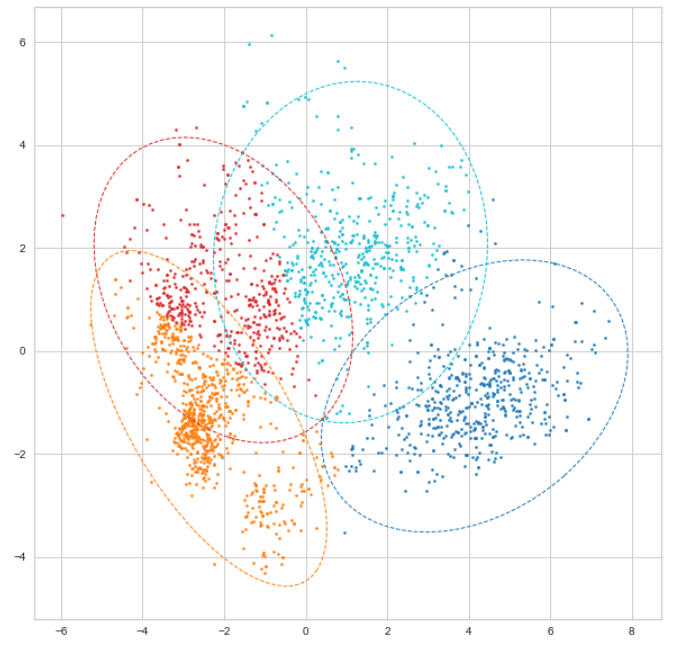
\includegraphics[width=.3\linewidth]{figures/FuzzyCMeans_clusters.PNG}\hfill
  \end{subfigure}
  \caption{Left to Right - Agglomerative, K-Means, Fuzzy C-Means}
\end{figure}

\begin{figure}[H]
  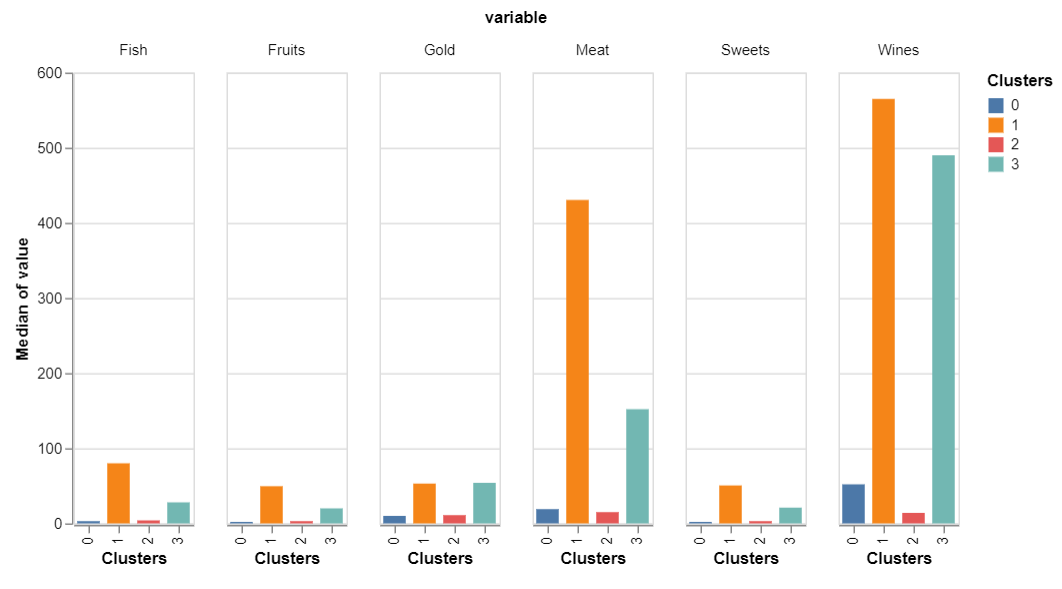
\includegraphics[width=\linewidth]{figures/Clusters_consumption.PNG}\hfill
  \caption{Consumption of Products}
\end{figure}
\noindent Both Agglomerative and Apriori methods identified Cluster 1 and Cluster 3 as the biggest consumers. The difference was much larger in the Meat and Wines department. \\

\noindent The Agglomerative, K-means, and Fuzzy C-means clustering methods all separated the data into very similar clusters. The three clustering methods yielded similar results due to the dataset's small size and uniformity. Nevertheless, we were able to pinpoint clear differences between the three methods.\\

\noindent The clusters yielded from Fuzzy C-means overlapped more so it’s more difficult to profile compared to Agglomerative and K Means. Because customer segmentation relies on clear results, Fuzzy C-means would not be the best to use.\\

\begin{figure}[H]
  \begin{subfigure}{0.48\textwidth}
    \centering
    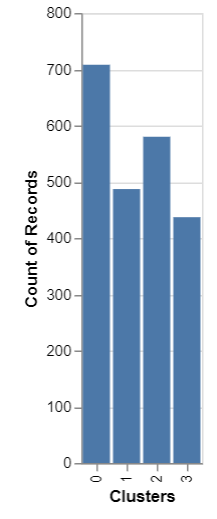
\includegraphics[scale = 0.5]{figures/Agglomerative_distribution.PNG}
    \caption{Agglomerative distribution}
  \end{subfigure}
  \begin{subfigure}{0.48\textwidth}
    \centering
    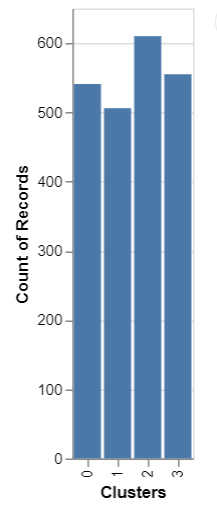
\includegraphics[scale = 0.5]{figures/KMeans_distribution.PNG}
    \caption{K-Means distribution}
  \end{subfigure}
  \caption{}
\end{figure}

\noindent Surprisingly, K-means yielded a more even distribution of cluster members than Agglomerative. For the former, Clusters 0, 2, and 3 were similar in size, with a larger difference between Cluster 1 and 2 of approximately 100 data points. The latter had differing cluster sizes, with a very large difference between Cluster 0 and 3 of over 250 data points. From figure 5, the difference in distribution for Agglomerative was larger than the difference for K-means. Thus, K-means is concluded to be the 'best' ML technique here.\\

\noindent These results go against the literature reviews. We postulate that our results are due to the nature of Agglomerative Clustering. Because it builds multiple minuscule clusters early on, the possibility remains that some undetected outliers may have interfered with the clustering formation. Given the small size of the dataset at around 2200 points, likely much smaller than the literature reviews' data, even a few outliers would influence the outcome.\\

\noindent Had our dataset been a larger size of 10000 points, the outcomes would be more consistent with the literature reviews. Agglomerative would likely out-perform K-means.\\

\begin{figure}[H]
  \centering
  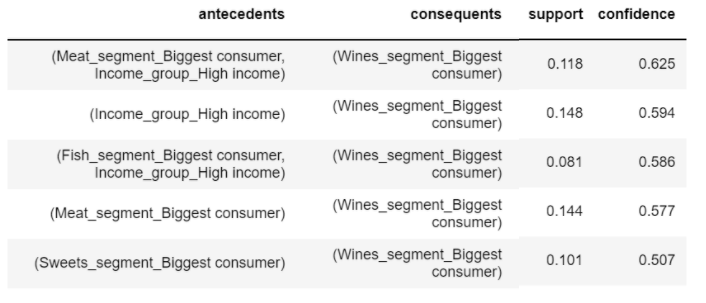
\includegraphics[width=.5\linewidth]{figures/Apriori_Algorithm.PNG}\hfill
  \caption{Apriori Table}
\end{figure}
\noindent The Apriori Algorithm’s table could be difficult to understand, since the support and confidence values were hard to understand/compare on their own. Due to this, Apriori was not the best ML method for this clustering application.\\

\section{Conclusion and Discussion}
The demand for product advertisement oriented towards specific customer markets was the inspirational basis for this project. Big Tech such as Amazon and Apple heavily rely on Machine Learning to focus their marketing on key customers. \\

\noindent Our main objective was determining which customers consumed the highest amounts of food products, in this case Wines and Meats.\\

\noindent The project pipeline entailed cleaning the dataset and removing invalid data, identifying general associations and trends within the dataset, then applying Agglomerative Clustering, Apriori Algorithm, K-Means, and Fuzzy C-Means to determine the clusters.\\

\noindent Our results indicated that Agglomerative clustering and K-means clustering yielded the most distinct clustering, and the most impactful attribute was Income. The latter yielded a more even distribution, so K-means is the winner.\\

\noindent Several interesting correlations were discovered. Education level did not meaningfully impact income amongst all clusters. Higher ages generally meant higher income (excluding highest earners [cluster 1]). In addition, more than 95\% of the customers in the highest-earning cluster [cluster 1] did not have children, despite ages ranging fairly equally from 20 - 80 years old.\\

\noindent When running the code, differing results may occur. Our team attempted to use seed arguments to force same results every time, but the Agglomerative results still vary. The K-means is consistent, although the ordering of the clusters will switch. We suspect the random results may be due to the nature of hierarchical clustering algorithms.

\section{References}
Ekhlassi, A., Nezhad, M., Far, S. et al. The relationship between brand personality and customer personality, gender and income: A case study of the cell phone market in Iran. J Target Meas Anal Mark 20, 158–171 (2012). https://doi.org/10.1057/jt.2012.12 \\

\noindent Phan Duy Hung, Nguyen Thi Thuy Lien, and Nguyen Duc Ngoc. 2019. Customer Segmentation Using Hierarchical Agglomerative Clustering. In Proceedings of the 2019 2nd International Conference on Information Science and Systems (ICISS 2019). Association for Computing Machinery, New York, NY, USA, 33–37. DOI:https://doi.org/10.1145/3322645.3322677 \\

\noindent S. H. Shihab, S. Afroge and S. Z. Mishu, "RFM Based Market Segmentation Approach Using Advanced K-means and Agglomerative Clustering: A Comparative Study," 2019 International Conference on Electrical, Computer and Communication Engineering (ECCE), 2019, pp. 1-4, doi: 10.1109/ECACE.2019.8679376.

\end{document}

